%
% 1-problem.tex
%
% (c) 2023 Prof Dr Andreas Müller
%
\section{Problemstellung
\label{buch:variation:section:problemstellung}}
\kopfrechts{Problemstellung}
Das Brachistochronenproblem, welches Johann Bernoulli im Jahr 1696
gestellt hat, war nicht das erste Optimierungsproblem für eine 
gesuchte Funktion, welches Physiker betrachtet haben.
Aber es darf als Ausgangspunkt für die Entwicklung der Variationsrechnung
betrachtet werden.
Alle diese Probleme zeichnen sich dadurch aus, dass Extremwerte
einer Grösse, die von allen Werten einer unbekannten Funktion abhängt,
gefunden werden sollen.
Die von Euler und Lagrange entwickelte Theorie zeigt, dass eine
Lösung für diese globale Eigenschaft immer auf eine lokale Bedingungen,
genauer auf eine Differentialgleichung reduziert werden kann, für deren
Lösung bereits eine ausgefeilte Theorie existiert.

%
% Der Anfang: das Brachistochronenproblem von Bernoulli
%
\subsection{Der Anfang: Das Brachistochronenproblem von Bernoulli}
%
% brachistochronenproblem.tex -- Brachistochronenproblem
%
% (c) 2021 Prof Dr Andreas Müller, OST Ostschweizer Fachhochschule
%
\documentclass[tikz]{standalone}
\usepackage{amsmath}
\usepackage{times}
\usepackage{txfonts}
\usepackage{pgfplots}
\usepackage{csvsimple}
\usetikzlibrary{arrows,intersections,math}
\begin{document}
\def\skala{1}
\def\r{1.5}
\pgfmathparse{3.14159/180}
\xdef\m{\pgfmathresult}
\def\xwert#1{\r*((#1)*\m-sin(#1))}
\def\ywert#1{\r*(cos(#1)-1)}
\def\punkt#1{ ({\r*((#1)*\m-sin(#1))},{\r*(cos(#1)-1)}) }
\begin{tikzpicture}[>=latex,thick,scale=\skala]

\draw[color=gray!50] plot[domain=0:360,samples=360]
	({\r*((\x)*\m-sin(\x))},{\r*(cos(\x)-1)});

\draw[->] (-0.1,0) -- (10,0) coordinate[label={$x$}];
\draw[->] (0,0.1) -- (0,-3.5) coordinate[label={left:$y$}];

\draw ({\m*\r*180},0.05) -- ({\m*\r*180},-0.05);
\node at ({\m*\r*180},0) [above] {$\frac{\pi}2\mathstrut$};
\draw ({\m*\r*360},0.05) -- ({\m*\r*360},-0.05);
\node at ({\m*\r*360},0) [above] {$\pi\mathstrut$};

\draw[line width=0.2pt]  ({\xwert{60}},0) -- \punkt{60};
\node at ({\xwert{60}},0) [above] {$a\mathstrut$};
\draw ({\xwert{60}},0.05) -- ({\xwert{60}},-0.05);

\draw[line width=0.2pt]  ({\xwert{160}},0) -- \punkt{160};
\node at ({\xwert{160}},0) [above] {$b\mathstrut$};
\draw ({\xwert{160}},0.05) -- ({\xwert{160}},-0.05);

\draw[color=red,line width=1.2pt] plot[domain=60:160,samples=100]
	({\r*((\x)*\m-sin(\x))},{\r*(cos(\x)-1)});

\fill[color=red] \punkt{60} circle[radius=0.08];
\node at \punkt{60} [above right] {$A$};
\fill[color=red] \punkt{160} circle[radius=0.08];
\node at \punkt{160} [below] {$B$};
\fill[color=red] \punkt{100} circle[radius=0.08];
\node at \punkt{100} [below left] {$M$};

\end{tikzpicture}
\end{document}


Im Jahr 1696 publiziert der Basler Mathematiker Johann Bernoulli, damals
Professor für Mathematik in Groningen das folgende Problem in der
von Leibniz herausgegebenen Zeitschrift {\em Acta eruditorum}:
\begin{center}
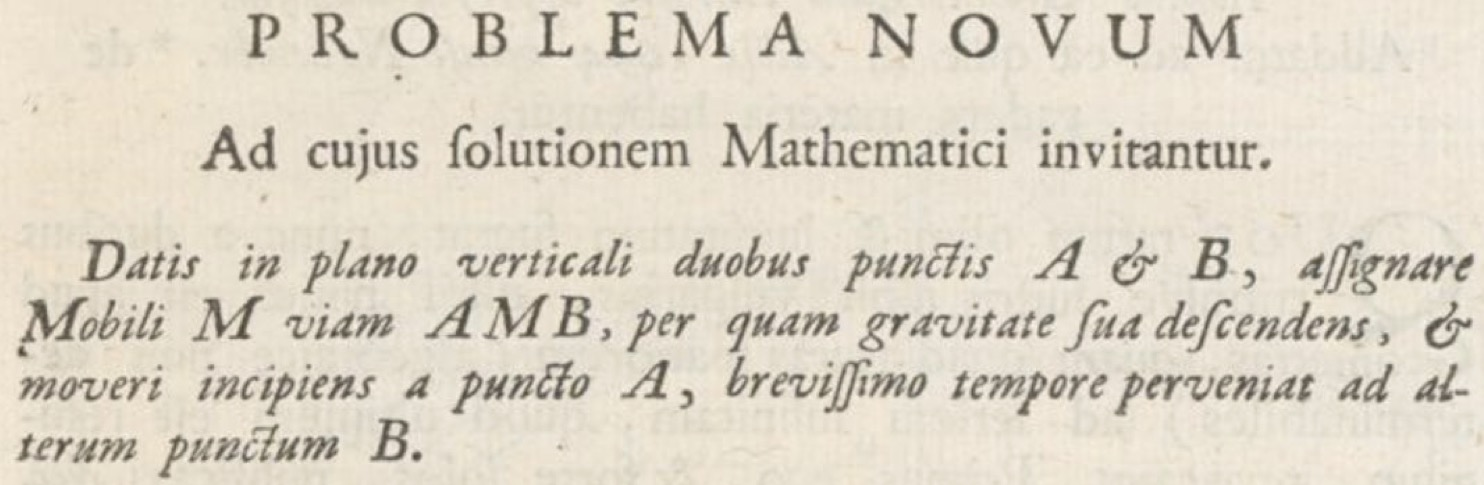
\includegraphics[width=0.8\textwidth]{chapters/020-variation/images/latein.jpg}
\end{center}
Zu deutsch:
\begin{quote}
Neue Aufgabe, zu deren Lösung die Mathematiker eingeladen werden.
Gegeben zwei Punkte $A$ und $B$ in einer vertikalen Ebene, finde
die Bahn $AMB$ eines Punktes $M$, der unter der Wirkung seines
Gewichtes in kürzester Zeit vom Punkt $A$ zum anderen Punkt $B$ absteigt.
\end{quote}
Die Situation der Aufgabenstellung ist in
Abbildung~\ref{buch:variation:fig:brachistochronenproblem}
dargestellt.
Bernoulli hat als Lösung gefunden, dass die Kurve eine Ausschnitt
aus einer Zykloide (in der Abbildung grau) sein muss.
Seine Lösung beruhte auf der Beobachtung, dass sich das Problem analog
zu einem Lichtausbreitungsproblem ist, für welches Fermat bereits
eine Lösung gefunden hat.

Da die Reibung vernachlässigt wird, ist die Energie des Massepunktes
erhalten.
Sie setzt sich aus der potenziellen und der kinetischen Energie
zusammen.
Die potenzielle Energie ist $-mgy$, die kinetische Energie ist
$\frac12mv^2$.
Die Energieerhaltung wird daher zu
\[
E=\frac12mv^2-mgy
\qquad\Rightarrow\qquad
v
=
\sqrt{2g}\!\sqrt{\frac{E}{gm}+y}
=
\!\sqrt{2(C+y)}.
\]
Durch Wahl einer anderen Zeiteinheit kann die Gleichung noch weiter
vereinfacht zu
\(
v = \sqrt{C+y}
\)
vereinfacht werden.
Gesucht ist also die zeitlich kürzeste Bahn eines Teilchens, 
dessen Geschwindigkeit auf bekannte Art $v(y)$ von der vertikalen
Koordinate abhängt.

%
% Das Fermat-Problem
%
\subsection{Das Fermat-Prinzip}
Bereits Fermat hat erkannt, dass das Brechnungsgesetz von Snellius
als Lösung eines Extremalproblems verstanden werden kann.

\begin{satz}[Fermat]
Sie $c/n_i$ die Geschwindigkeit, mit der sich Licht im Medium $M_i$
ausbreitet.
Ein Lichtstrahl von $A_1$ nach $A_2$ geht durch denjenigen Punkt $B$ 
auf der Grenzfläche zwischen den Medien, für den sich die Sinus der
Winkel $\alpha_i$ zwischen den Strahlen und der Normalen zur Grenzfläche
umgekehrt wie die $n_i$ verhalten, wenn also das Brechungsgesetz
\[
\frac{\sin\alpha_1}{\sin\alpha_2}
=
\frac{n_2}{n_1}
\]
gilt.
\end{satz}

\begin{proof}
Ohne der Beschränkung der Allgmeinheit können wir auf die Betrachtung
einer Ebene beschränken, die die beiden Punkte $A_i$ enthält und senkrecht
auf der Grenzfläche steht.
Wir dürfen weiter annehmen, dass die $x$-Achse in der Grenzfläche liegt 
und die Punkte $A_i$ die Koordinaten $(x_i,y_i)$ und der Punkt $B$ die
Koordinaten $(x,0)$ hat.
Es ist derjenige Punkt $x$ zu bestimmen, für den die Lichtzeit entlang 
des Pfades $A_1BA_2$ minimal wird.
Diese Zeit ist
\begin{align*}
t
&=
\frac{\overline{A_1B}}{c/n_1}
+
\frac{\overline{BA_2}}{c/n_2}
\\
ct
&=
n_1\overline{A_1B}
+
n_2\overline{A_2B}
\\
&=
n_1\!\sqrt{(x-x_1)^2 + y_1^2}
+
n_2\!\sqrt{(x_2-x)^2 + y_2^2}
\end{align*}
Das Minimum wird bei einer Nullstelle der Ableitung nach $x$ gefunden,
also bei einer Lösung der Gleichung
\begin{align*}
0
&=
n_1\frac{2(x_1-x)x}{\sqrt{(x_1-x)^2+y_1^2}}
+
n_2\frac{-2(x-x_2)x}{\sqrt{(x_2-x)^2+y_2^2}}.
\intertext{Indem man den zweiten Term auf der rechten Seite auf die linke
Seite bringt und durch $x$ dividiert, erhält man}
n_1
\frac{x_1-x}{\sqrt{(x_1-x)^2+y_1^2}}
&=
n_2
\frac{x-x_2}{\sqrt{(x_2-x)^2+y_2^2}}.
\end{align*}
Der Nenner ist auf beiden Seiten die Hypothenuse eines rechtwinkligen
Dreiecks, welches als Ankathete die Normale zur Grenzfläche hat.
Der Zähler ist die Gegenkathete des Winkels $\alpha_i$ zwischen der
Hypothenuse und der Normalen.
Daher ist der Quotient der Sinus des Winkels oder
\begin{equation}
n_1 \sin\alpha_1 = n_2 \sin\alpha_2.
\label{buch:variation:problem:eqn:snelliusinvariante}
\end{equation}
Die Gleichung~\eqref{buch:variation:problem:eqn:snelliusinvariante}
ist gleichbedeutend mit dem Brechungsgesetz
\[
\frac{\sin\alpha_1}{\sin\alpha_2}
=
\frac{n_2}{n_1}
\]
von Snellius.
\end{proof}

Der Satz von Fermat etabliert das Brechungsgsetz also Lösung eines
Extremalproblems.
Die Natur wählt für einen Lichtstrahl den zeitlich kürzesten Weg.
Der Beweis des Satzes von Fermat zeigt, dass entlang des Lichtstrahls
an jeder Grenzfläche zwischen Medien die Bedingung
\eqref{buch:variation:problem:eqn:snelliusinvariante}
erfüllt.
Wenn die optische Dichte $n$ eine Funktion von $n(y)$ ist, dann
wird der Lichtstrahl nicht nur in diskreten Punkten geknickt, sondern
entlang des ganzen Strahles gekrümmt.
Folgt der Strahl der Kurve $x(y)$, die mit der vertikalen den Winkel
$x'(y) = \tan\alpha(y)$ einschliesst.
Damit lässt sich auch die Sinus-Funktion ausdrücken, es gilt
\[
\sin\alpha(y)
=
\frac{x'(y)}{\pm\!\sqrt{x'(y)^2+1}}.
\]
Aus der Form~\eqref{buch:variation:problem:eqn:snelliusinvariante}
des Brechungsgesetztes wird dann die Gleichung
\begin{equation}
n_1\sin\alpha(y)
=
\frac{n_1(y)x'(y)}{\pm\!\sqrt{x'(y)^2+1}}
=
\operatorname{const}
\qquad\Rightarrow\qquad
\frac{n_1(y)^2x'(y)^2}{x'(y)^2+1}=C.
\label{buch:variation:eqn:fermatdgl}
\end{equation}
Dies ist eine Differentialgleichung für die Funktion $x(y)$.
Sie kann auch in die Form
\[
x'(y)^2
=
\frac{C}{(n_1(y)^2-C)}
\]
gebracht werden.

%
% Das Brachistochronenproblem als Lichtausbreitungsproblem
%
\subsubsection{Das Brachistochronenproblem als Lichtausbreitungsproblem}
Das Fermat-Prinzip besagt, dass ein Lichtstrahl, der sich in einem Medium
mit der Geschwindigkeit $c/n(y)$ ausbreitet, die Gleichung 
\eqref{buch:variation:eqn:fermatdgl} erfüllt.
Beim Brachistochronenproblem ist die Geschwindigkeit $v(y)=\!\sqrt{C-y}$ und 
damit $n(y) = c/\!\sqrt{C-y}$.
Eine Brachistochrone ist also eine Kurve, die die aus
\eqref{buch:variation:eqn:fermatdgl} folgende Gleichung
\begin{equation}
\frac{x'(y)^2}{(1+x'(y)^2)(C-y)} = K
\label{buch:variation:problem:eqn:bernoullidgl}
\end{equation}
erfüllen.

%
% Die Bernoullische Lösung
%
\subsubsection{Die Bernoullische Lösung}
Bernoulli hat gefunden, dass die Brachistochrone ein Zykloidenbogen ist.
Dies lässt sich dadurch verifizieren, dass man die Parametrisierung
einer Zykloide in die
Gleichung~\eqref{buch:variation:problem:eqn:bernoullidgl}
einsetzt.
Die Zykloide hat die Parametrisierung
\[
\left.
\begin{aligned}
x &= r(\varphi - \sin\varphi) 
\\
y &= r(1-\cos\varphi)
\end{aligned}
\right\}
\quad
\text{mit der Ableitung}
\quad
\left\{
\begin{aligned}
\dot{x}(\varphi) &= r(1-\cos\varphi)\\
\dot{y}(\varphi) &= r\sin\varphi
\end{aligned}
\right.
\]
für $\varphi\in\mathbb{R}$.
Die Ableitung ist
\[
x'(y)
=
\frac{\dot{x}(\varphi)}{\dot{y}(\varphi)}
=
\frac{1-\cos\varphi}{\sin\varphi}.
\]
Eingesetzt in \eqref{buch:variation:problem:eqn:bernoullidgl}
wird daraus
\[
\frac{\dot{x}(\varphi)^2}{
(\dot{y}(\varphi)^2 +\dot{x}(\varphi)^2)
(C-r(1-\cos\varphi))
}
=
\frac{(1-\cos\varphi)^2}{
((1-\cos\varphi)^2+\sin^2\varphi)
(C-r+r\cos\varphi)
}
=
K.
\]
Ausmultiplizieren im Nenner ergibt
\[
\frac{(1-\cos\varphi)^2}{
(1-2\cos\varphi+\cos^2\varphi+\sin^2\varphi)
(C-r+r\cos\varphi)
}
=
\frac{1-\cos\varphi}{
2(C-r+r\cos\varphi)
}
\]

%
% Das Brachistochronenproblem als Variationsproblem
%
\subsection{Das Brachistochronenproblem als Variationsproblem}
Die Bernoullische Lösung des Brachistochronenproblems verwendet die
Analogie zum Fermat-Prinzip.
Eine solche Analogie ist nur selten möglich, daher soll das Problem
jetzt in eine Form gebracht werden, in die auch viele ähnliche
Optimierungsproblem gebracht werden können.

Wir erinnern daran, dass die Geschwindigkeit des Massepunktes durch
$v(y)=\sqrt{C-y}$ gegeben ist.
Damit lässt sich die Zeit berechnen, die der Massepunkt entlang der
Lösungskurve braucht, wenn man diese als Funktion $y(x)$ mit beschreibt.
Die Punkte $A$ und $B$ sollen die $x$-Koordinaten $a$ bzw.~$b$ haben.
Für das Kurvenstück zwischen den $x$-Koordinaten $x$ und $x+\Delta x$
braucht der Massepunkt die Zeit
\[
\frac{ \sqrt{\Delta x^2 + \Delta y^2} }{v(y)}
=
\frac{ \sqrt{1 + y'(x)^2} }{ v(y) } \Delta x.
\]
Die Zeit ist das Integral
\begin{equation}
t
=
\int_a^b \frac{\sqrt{1+y'(x)^2}}{v(y(x))}\,dx
=
\int_a^b \sqrt{\frac{1+y'(x)^2}{C-y(x)}}\,dx.
\label{buch:variation:problem:eqn:brachint}
\end{equation}
Der Integrand auf der rechten Seite hängt nur von den Funktion $y(x)$
und $y'(x)$ ab.
Dies kommt vor allem daher, dass die Geschwindigkeit nur von $y$ abhängt,
nicht auch noch von $x$.
Im Allgemeinen wird man also davon ausgehen müssen, dass der Integrand
auch noch von $x$ abhängt.
Die Variationsrechnung befasst sich mit Problemen, in denen Funktionen
gefunden werden müssen, die ein Integral wie das in
\eqref{buch:variation:problem:eqn:brachint}
minimiert oder maximiert werden müssen.

\begin{definition}[Lagrange-Funktion des Brachistochronenproblems]
Die Lagrange-Funk\-tion des Brachistochronenproblems ist der
Integrand des Integrals
\eqref{buch:variation:problem:eqn:brachint},
\index{Lagrange-Funktion}%
also die Funktion
\[
L(x,y,y')
=
\sqrt{\frac{1+y^{\prime 2}}{C-y}}.
\]
\end{definition}

%
% Funktionale
%
\subsection{Funktionale}


